\begin{figure}[h]
    \centering
    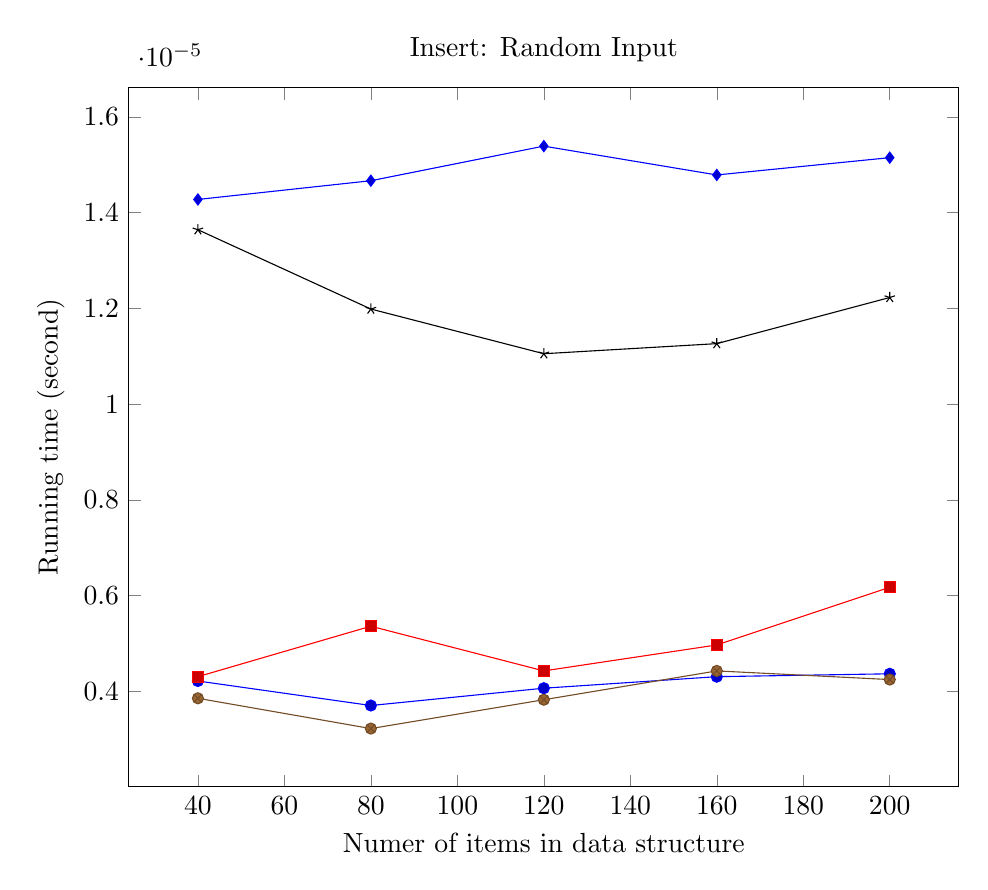
\begin{tikzpicture}
        \begin{axis}[
            xlabel={Numer of items in data structure},
            ylabel={Running time (second)},
            title={Insert: Random Input},
            width=\textwidth
        ]
		\addplot coordinates {
			(200, 4.367042383179864e-06)
			(160, 4.3068073157570556e-06)
			(120, 4.065867046065818e-06)
			(80, 3.704456641884235e-06)
			(40, 4.216454714622841e-06)
		};
		\addplot coordinates {
			(200, 6.17409440337724e-06)
			(160, 4.969393056342142e-06)
			(120, 4.427277450247402e-06)
			(80, 5.36092099423513e-06)
			(40, 4.3068073157570556e-06)
		};
		\addplot coordinates {
			(200, 4.246572248334246e-06)
			(160, 4.427277450247402e-06)
			(120, 3.824926776729854e-06)
			(80, 3.2225761032123047e-06)
			(40, 3.855044310085987e-06)
		};
		\addplot coordinates {
			(200, 1.2227718672264132e-05)
			(160, 1.1263957594564999e-05)
			(120, 1.1053134858585168e-05)
			(80, 1.1986778402572894e-05)
			(40, 1.364324275492379e-05)
		};
		\addplot coordinates {
			(200, 1.5149119438717661e-05)
			(160, 1.4787709034536078e-05)
			(120, 1.5390059708053626e-05)
			(80, 1.466723889969046e-05)
			(40, 1.4275710962152743e-05)
		};
        \legend{}
        \end{axis}
    \end{tikzpicture}
    \caption{Average of 0 operations, benchmarked every 0, starting at 0.}
\end{figure}